 \section*{Решения и комментарии}

\subsubsection*{Определение большинства}% (IDENTIFYING THE MAJORITY)

Идея состоит в том, что каждый раз, когда на счётчике появляется 0 (начальная позиция), 
вы запоминаете имя, которое слышите в данный момент, и добавляете на счётчике 1.
Когда на счётчике больше, чем 0, вы прибавляете, если имя, которое вы слышите то же, что вы держите в уме.
В противном случае отнимаете на счётчике 1, но сохраняете в уме прежнее имя.

Возможно, конечно, закончить с именем, которое называлось только один раз (например, если список был «Алиса, Боб, Алиса, Боб, Алиса, Боб, Чарли»).
Тем не менее, если имя появлялось больше, чем половину раз, то оно гарантированно сохранится у вас в уме до конца.
Причина того, что имя останется в вашей памяти, состоит в том, что на счётчике больше прибавляется, чем отнимается.

Данный алгоритм описан в статье Майкла Фишера и Стивена Зальцберга.\footnote{M. J. Fischer, S. L. Salzberg, ``Finding a Majority Among n Votes''. \emph{Journal of Algorithms} Vol. 3, No 4 (December 1989), pp 362--380}

\subsubsection*{Обездвиживатель Конвея}% (THE CONWAY IMMOBILIZER)

Непросто придумать алгоритм, который избегает зацикливания и не делает глупостей близко цели.
В данной задаче сработает следующий трюк.

\medskip

Если есть пустая колода, то перекладываем в неё карту из колоды слева (возможно по кругу) кроме следующих двух случаев К, --- , Т и К, Т, ---, в которых следует положить туза на короля.

Далее, если все карты открыты и дама находится в левой колоде, то кладём короля на даму, в противном случае, карту справа от дамы перекладываем в колоду справа от неё (опять же, возможно по кругу).

Очевидно, что если какой-то ход собирает три карты в колоду, то получена выигрышная комбинация.
Начав с комбинации две-пусто, даже такой, как К, ---, Т или
К, Т, ---, все карты откроются максимум за три хода (если только игра не закончится).
\begin{figure}[h!]
\centering
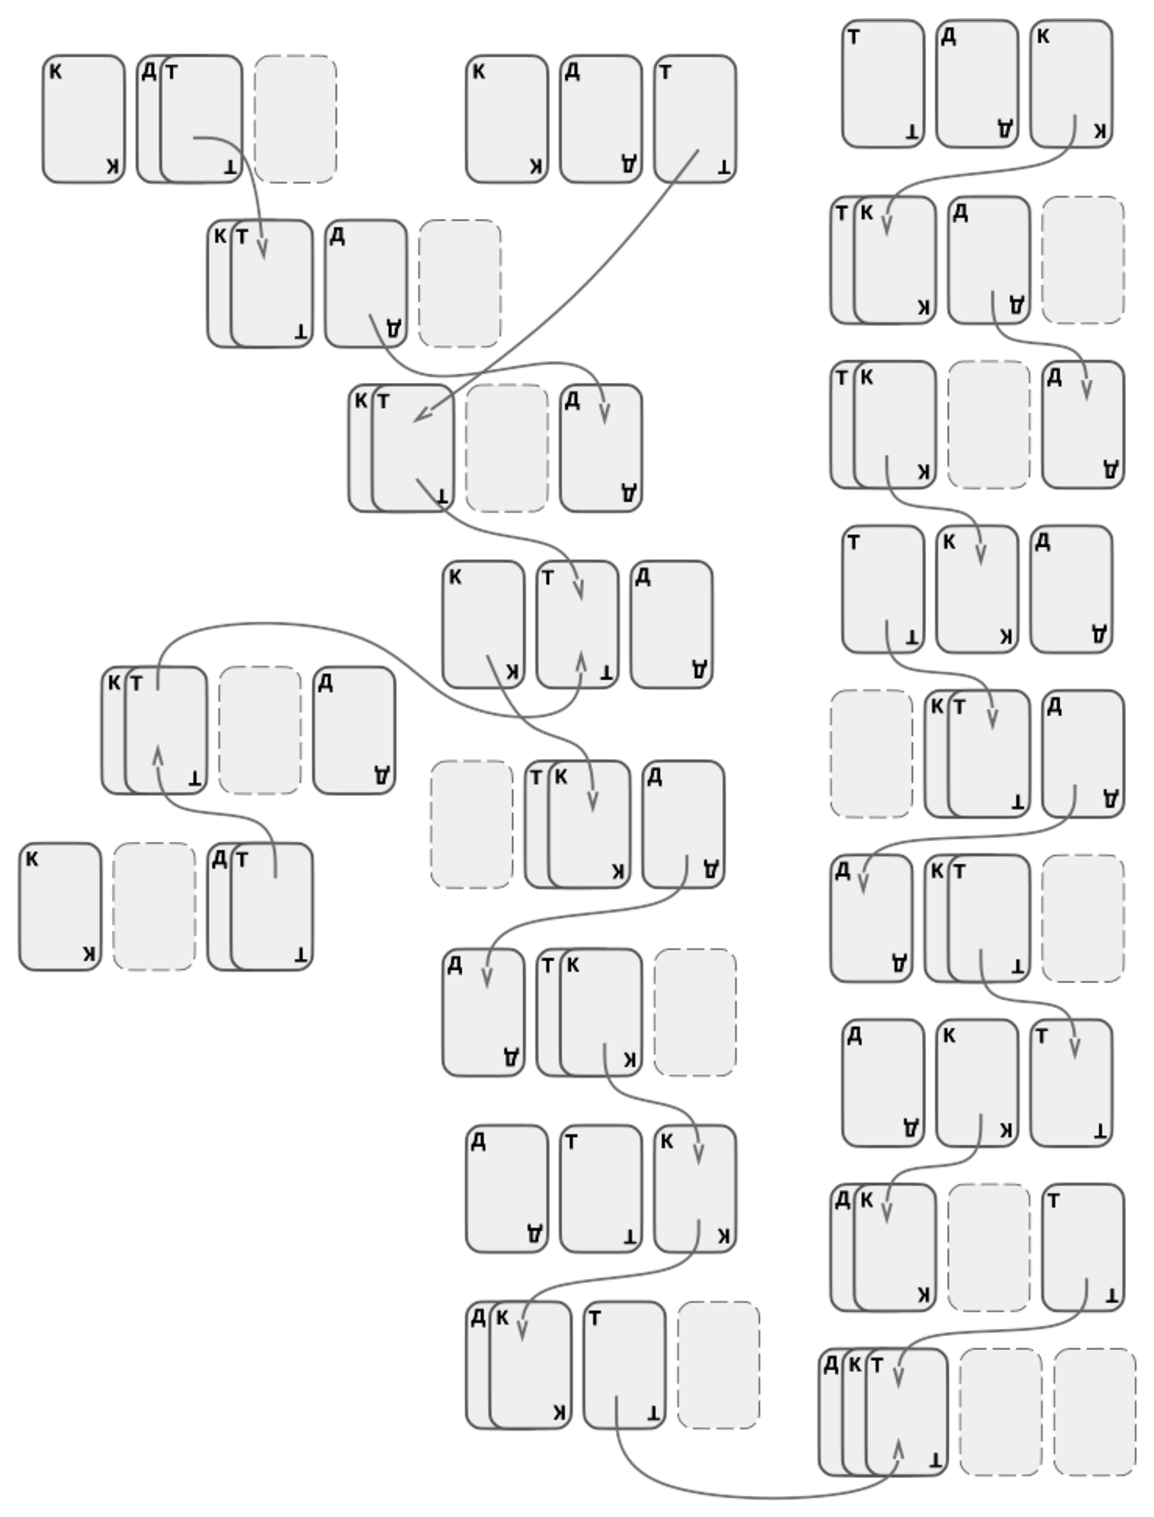
\includegraphics[scale=0.55]{Figs/Handicaps/conway-ru}
\end{figure}
Таким образом, достаточно проверить, что все шесть возможных комбинаций открытых карт приводят к победе  (см. диаграмму).
\heart

Удивительным образом, этот алгоритм можно обобщить для работы с любым (фиксированным, известным) числом карт, оперируя всё теми же тремя колодами.
Скажем, для 52 карт, пронумерованных от 1 до 52, следующие правила (данные в приоритетном порядке) в конечном итоге приведут к тому, что слева окажется колода, сложенная по-порядку с 1-ой картой наверху.

\begin{enumerate}[(1)]
\item Если видим 2, 1, ---, то кладём $1$-ю на $2$-ю;
\item Если видим две произвольные карты, ---, то перекладываем карту вправо (возможно по кругу) в пустую колоду;
\item Если видим $k$, $j$, $k-1$, при $j < k$, то кладём $(k-1)$-ю на $k$-ю;
\item Если видим только одну карту, то перекладываем карту налево;
\item Если видим три карты, то карту справа от наибольшей перекладываем дальше направо.
\end{enumerate}

Докажем, что этот алгоритм действительно работает.
Предположим, что мы видим карту 52 в средней или в правой колоде.
Тогда, следуя правилу (2) и (5), она в итоге окажется в левой колоде а все остальные карты попадут в среднюю.
По мере их перемещения вправо согласно правилу (2), карты $51, 50, 49, \dots, k$ будут складываться на $52$-ю согласно правилу (3) для некоторого $k < 52$, и средняя колода опустеет.
Разумеется, если $k = 1$, то задача решена --- последний ход сделан по правилу (1).
В противном же случае $k$-я карта переместится в среднюю колоду по правилу (2) и в правую по правилу (5), за ней аналогичным образом последует $(k+1)$-я, и так далее, пока в правой колоде не окажется 51 карта, верхние карты которой упорядочены от $51$-й до $k$-й.

Теперь $52$-я карта перекладывается в среднюю колоду,
а правая колода перекладывается в обратном порядке в левую.
Далее $52$-я карта передвигается в правую колоду, а левая колода перемещается в среднюю колоду, снова меняя порядок.
Наконец $52$-я карта перекладывается обратно в левую колоду.
В этот момент в средней колоде окажутся карты от $51$-й до $k$-й, с $51$-й наверху.
Дальше карты с $51$-й по $k$-ю перемещаются согласно правилу (2) направо и оказываются в левой колоде по правилу (3), до тех пор пока, опять, $k$-я, $(k+1)$-я, $\dots, 52$-я не попадут в левую колоду.

Правая колода сейчас пустая, следовательно, $(k-1)$-я карта находится где-то в средней.
Если она не в самом низу, то ей придётся перейти в левую колоду и процесс, описанный выше, повторится для некоторого $k'<k$.
Если же случилось, что $(k-1)$-я карта оказалась в самом низу, то она не попадёт влево (если только, она не $1$-я), потому что, когда она переместится вправо по правилу (5), средняя колода опустеет, и мы вынуждены применить правило (2) вместо (3).
Однако, в конце следующего цикла, в средней колоде будет обратный порядок, с картой $k-1$ наверху.
Отсюда следует, что значение $k$ уменьшается хотя бы каждый второй раз, как $52$-я карта попадает в пустую левую колоду.

Для завершения доказательства, нам осталось проверить, что в какой-то момент $52$-я карта появится на верху средней или правой колоды. %???
Предположим, что $52$-я появилась на левой колоде (все остальные карты под ней).
Следуя правилу (3), она может собрать над собой $51$-ю, $50$-ю, $\z\dots, k$-ю, а остальные карты окажутся в средней и, возможно, в правой колоде.
Затем правила (2) и (5) опустошат среднюю колоду.
Далее $k$-я карта переместится в середину и потом вправо, затем, аналогично, $(k+1)$-я, и так далее (как и выше), пока $52$-я снова не окажется наверху, но на этот раз (после того, как $51$-я перешла в правую колоду) средняя колода будет пустая.
Значит $52$-я кладётся на среднюю, и мы получаем желаемую конфигурацию.

\subsubsection*{Крутящиеся выключатели}% (SPINNING SWITCHERS)

Эта задача попала ко мне от Саши Барга из Мэрилендского университета, но, похоже, что в этот момент она была уже много где известна.
Как и во многих других задачах, окажется полезным рассмотреть сначала более простой её вариант.

Рассмотрим версию с двумя выключателями: нажав на обе кнопки, мы выясним, находились ли они в одинаковом состоянии, если да, то лампочка загорится (если она уже не горела).
В противном случае, на следующем шаге нажмём одну кнопку, после этого кнопки \emph{будут} в одинаковом состоянии, и в наихудшем случае нам придётся сделать ещё один шаг, нажав сразу обе кнопки, чтобы лампочка наконец зажглась.

Вернёмся к варианту с четырьмя лампочками.
Обозначим через 
А операцию, когда мы нажимаем все четыре кнопки, 
D --- диагональные кнопки, 
N --- соседние и 
S --- одну кнопку.
Тогда последовательность операций ADANASADAND включит лампочку максимум за 12 шагов.

В более общем виде для выключателей в углах $n=2^k$-угольника это можно проделать за $2^{n}-1$ шаг следующим образом.
Пусть $X\z=X_1,\dots,X_m$ шаги для $\tfrac n2=2^{k-1}$-угольника.
Составим из противоположных выключателей пары, если $X_i$ --- шаг для $\tfrac n2$-угольника, при котором нажимаются кнопки $i_1,\dots,i_j$, тогда пусть $X_i'$ будет шагом для $n$-угольника, при котором нажимаются кнопки $i_1,\dots,i_j$ и $i_1+\tfrac n2,\dots,i_j+\tfrac n2$.
Пусть $X'$ обозначает последовательность шагов $X_1',\dots,X_m'$.

Нам также необходим шаг $X_i''$ для $n$-угольника, при котором нажимаются только кнопки $i_1,\dots,i_j$.

Будем говорить про противополжную пару, что она «чётная», если оба выключателя включены или оба выключены.
Если все пары чётные, тогда последовательность шагов $X'$ включит лампочку.
Идея в том, чтобы посредством применения шагов $X_1''$, $X_2''$ и так далее, сделать все пары чётными, каждый раз проверяя при помощи $X'$, добились ли мы успеха.
Порядок шагов такой:
\begin{align*}
X_1',\dots,X_m';X_1'';X_1',\dots,X_m';X_2'';
\\
X_1',\dots,X_m';\dots,:X_m'';X_1',\dots,X_m',
\end{align*}
или, более компактно: $X';X_1'';X',X_2'';X';\dots,X_m'',X'$.
Всего получилось $(m+1)m+m=m(m+2)$ шагов.
Следовательно, если $f(n)$ означает число шагов, предпринятых для решения $n$-угольника, то 
$f(n)=f(\tfrac n2)(f(\tfrac n2)+2)$,
и поскольку $f(1)=2^1-1=1$, получаем, что $f(n)=2^n-1$ если $n$ степень двойки.

Эта последовательность действий работает, потому что шаги типа $X''$ работают на чётных/нечётных парах также, как и шаги типа $X$ работали на включенных/выключенных парах, и, между тем, шаги типа $X'$ абсолютно не влияют на конфигурацию чётных/нечётных пар.
\heart

С другой стороны, задача не разрешима, если $n$ не является степенью двойки, например, если $n=m2^k$, при нечётном $m>1$.
Для представления одновременно конфигурации выключателей (1 = «включен», 0 = «выключен») и операции (1 = «нажать», 0 = «не трогать») можно прибегнуть к бинарным векторам длины $n$.
Пусть $v$ такой вектор, обозначим через $v^i$ результат его вращения на $i$ шагов вправо.
Применение операции $w$ к конфигурации $v$ приведёт к конфигурации $v+w$, если поворота не было, но поскольку поворот был, мы получаем $v+w^i$ для некоторого значения $i$.

Будем говорить, что $n$-вектор $v$ является «неровным», % [rough ?], 
если число различных его вращений $v^0,v^1,\dots,v^{n-1}$ не равно степени двойки.
Предположим (как и в начале), что до применения операции возможна \emph{любая неровная конфигурация с точностью до вращения}.
Мы утверждаем, что после любой фиксированной операции $w$ все ещё возможна \emph{любая неровная конфигурация с точностью до вращения}.
Таким образом нет гарантированного способа избавится от неровных конфигураций и, в частности, нельзя гарантировать получения $11\dots1$.

Для нечётного $n$, то есть при $n=m$, все векторы, кроме $00\dots0$ и $11\dots1$ неровные.
Если $w$ некий вектор и $v$ неровный вектор, то $v-w$ (то же что и $v+w$), или $v-w^1$ будут неровными, так что, если одно из вращений векторов $v-w$ или $v-w^1$ было возможно до применения операции, то вращение $v$ возможно после её применения.

Если $n=m2^k$, при $k>1$, то можно разбить $n$-цикл на сегменты длины $2^k$; вектор $v$ будет неровным если только он не одинаков на всех сегментах.
Следовательно, если вектор $v$ неровный, то существует $1\le j\le 2^k$, что его координаты $i2^k+j$ для $1\le j\le m$ не все равны.
И остаётся применить рассуждение выше, к векторам $v-w$ и $v-w^{2^k}$.

\subsubsection*{Комната с одной лампочкой}% (THE ONE-BULB ROOM)

Я услышал эту задачу от Адама Чэлкрафта, %(Adam Chalcraft)
который имеет честь представлять Великобританию на международных соревнованиях по одноколёсному хоккею.
Задача также появлялась на сайте www.ibm.com и была перепечатана в Emissary --- информационном бюллетене Математического института в Беркли. %(Matematical Science Research Institute) 
Одна из версий задачи появлялась даже в заслуженно известной программе Национального Общественного Радио «Car Talk» в 2003 году.

Однако, считаю нужным предупредить читателя, что эту задачу иногда путают с куда более сложной задачей, с которой вам предстоит встретиться в следующей главе.

\medskip

Безусловно, необходимо предположить, что между посещениями заключённых никто в комнате с лампочкой не балуется.
Заключённым необязательно знать, в каком состоянии изначально находится лампочка.

Идея заключается в том, что один из заключённых (скажем, Алиса) всё время пытается лампочку включить, а каждый из остальных выключает её \emph{два раза}.

Более подробно: Алиса всегда включает лампочку, если она выключена, в противном случае, оставляет её включённой.
Остальные заключённые выключают её первые два раза, если она включена, и оставляют её гореть при последующих посещениях.

Алиса считает, сколько раз она попадает в тёмную комнату после своего первого 
посещения, после $2n-3$ \emph{тёмных} визитов, она может заключить, что все побывали в комнате.
И вот почему:
Каждое тёмное посещение говорит о том, что один из остальных $n-1$ заключённых побывал в комнате.
Если же кто-то из них, скажем, Боб, не посещал комнаты, тогда лампочка не могла быть выключена больше, чем $2(n-2)\z=2n-4$ раз.
С другой стороны, Алиса в конце концов должна будет достичь её $2n-3$ тёмных визитов, потому что в итоге лампочка будет выключена $2(n-1)=2n-2$
раз и только одно из этих выключений (в случае если один из заключённых побывал в комнате до первого визита Алисы и выключил изначально горящую лампочку) может не засчитаться Алисой за тёмный визит.

Если заключённых только два, то каждый из них узнаёт о том, побывал ли другой в комнате, поскольку Алиса дожидается её первого тёмного повторного посещения, в то время как Боб ждёт свой первый \emph{светлый} повторный визит.
Однако, для для случая $n>2$ имеется доказательство того, что невозможно гарантировать, что более одного заключённого узнают посетили ли все остальные комнату.
Ниже приводится набросок этого доказательства.
Читателям рекомендуется его пропустить, если только им не интересно, как получаются отрицательные результаты в задачах о передаче информации.
Я включил это доказательство потому, что, насколько мне известно, оно нигде не появлялось.

По сути, мы утверждаем, что противник (который знает стратегию заключённых) может вынуждать их совершать только бесполезные действия, кроме тех, что применялись в протоколе выше.

Давайте сосредоточимся на одном заключённом, Алисе.
Мы предполагаем, что её стратегия детерминистическая и основана исключительно на последовательности состояний лампочки, которые она до сих пор наблюдала.

Предположим, что стратегия Алисы заставляет её (в некоторых обстоятельствах) изменить состояние лампочки, после того, как она нашла её в том же состоянии, что и во время своего последнего посещения.
Тогда противник может немедленно отправить её обратно в комнату, «сводя на нет» её предыдущий визит.
В результате, эта часть стратегии Алисы может только дать противнику дополнительную опцию.
Исходя из этого, можно предположить, что Алиса не должна менять состояние лампочки, если она находит её в том же виде, как оставила в свой последний визит.

Далее, предположим, что Алисе в некий момент требуется оставить лампочку в том же состоянии, в котором она её нашла.
Тогда мы утверждаем, что можно предположить, что после этого она никогда снова не предпримет каких-либо действий!
Почему?
Потому что, если противник не хочет, чтобы она продолжала действовать, то он может устроить так, что Алиса никогда не увидит лампочку в состоянии, отличном от того, которое она видит в данный момент.
Он может это сделать, поскольку, если Алиса действительно останется навсегда неактивной, то, по крайней мере, одно из состояний («включено» или «выключено») будет повторяться бесконечно часто.
Положим, это «выключено».
Тогда противник может составить расписание для Алисы так, что лампочка будет выключена как в её посещении сейчас, так и во всех последующих, и следовательно, согласно предыдущему рассуждению, она никогда не будет снова действовать.
Итак, ещё раз, в этом случае у противника есть возможность заставить Алису замолчать, и можно предположить, что ровно это он и делает.

Очевидно, Алиса не может начинать с инструкции оставить лампочку в том же состоянии, как она её находит, так как в этом случае она перестанет действовать совсем, и никто никогда не узнает, посещала ли она комнату.%
\footnote{Если только она не пользуется очень сильными духами...}
Скажем, она должна включить лампочку, если она выключена, в обратном случае оставить лампочку как есть.
Тогда она ничего не будет делать до тех пор, пока опять не попадёт в комнату с выключенной лампочкой, и в этом случае она может только снова включить лампочку или остаться бездейственной навсегда.
Таким образом, число раз, когда Алиса включает лампочку, ограничено неким $j$ (которое можно считать константой, иначе у противника будет больше преимуществ).
Назовём такую стратегию $+j$, где $j$ положительное целое число или бесконечность.
Аналогичное рассуждение, применённое для случая, когда Алиса должна во время первого визита выключить лампочку, приводит к стратегии $-j$.

Остаётся ещё один вариант, когда Алиса должна будет изменить состояние лампочки в свой первый визит в комнату, но в этом случае далее она вынуждена будет продолжить действовать так, как описано выше, в зависимости от того, включила она лампочку или выключила.
И это снова даёт противнику дополнительное преимущество.

Всё сводится к тому, что у каждого заключённого имеется стратегия $+j$ или $-j$ для различных $j$.
Если все они только выключают (или включают) лампочку, никто ничего не сможет определить.
Таким образом, можно предположить, что у Алисы стратегия $+j$, а у Боба $-k$.
Если Чарли включает лампочку, то Алиса никогда не сможет определить, закончили ли Боб или Чарли, или же у них остаётся ещё по одному заданию.
Если Чарли выключает лампочку, то тогда Боб --- это тот, кто останется в неведении.

Учитывая всё вышесказанное, мы получаем, что для того, чтобы какой-то заключённый смог определить, что все посетили комнату,
Алиса должна включать лампочку, в то время как все остальные выключать (или наоборот).
Действительно, если стратегия у Алисы $+j_1$, а у остальных  $-j_2,\dots,-j_n$, то легко проверить, что условие, при котором каждое $j_i$ конечно и не меньше 2, а $j_1$ больше, чем сумма остальных минус наименьший из них, является необходимым и достаточным.

Отсюда следует, что если $n>2$, тогда максимум одному заключённому гарантирована честь знать, все ли побывали в комнате.
Уфф!

\subsubsection*{Два шерифа}% (ТHE TWO SHERIFFS)

Если два шерифа (назовём их Лев и Ральф) обмениваются секретной информацией, они могут использовать этот секрет для того, чтобы зашифровать свой разговор и достичь цели.
Но так как они никогда прежде не встречались, им придётся \emph{изготовить} этот секрет.

\medskip

Предположим, что пары, к которым Лев и Ральф сузили свои списки подозреваемых, не одинаковы, то есть существует возможность определить убийцу.
В этом случае, если, скажем, Лев просто называет свою пару, то Ральф будет знать, кто убийца.
Но тогда и банда линчевателей будет знать всё, что знает Лев, так что любая попытка Ральфа сообщить Льву имя убийцы, без того, чтобы об этом не прознали линчеватели, обречена на провал.

Лев и Ральф должны подойти к определению имени убийцы более хитрым способом.
Составим таблицу из всех возможных пар подозреваемых таким образом, что каждый столбец содержит разбиение восьми подозреваемых на четыре пары.
Вот один из способов:

\[
\begin{matrix}
\{1,2\}&\{1,3\}&\{1,4\}&\{1,5\}&\{1,6\}&\{1,7\}&\{1,8\}
\\
\{3,4\}&\{2,4\}&\{2,3\}&\{2,6\}&\{2,5\}&\{2,8\}&\{2,7\}
\\
\{5,6\}&\{5,7\}&\{5,8\}&\{3,7\}&\{3,8\}&\{3,5\}&\{3,6\}
\\
\{7,8\}&\{6,8\}&\{6,7\}&\{4,8\}&\{4,7\}&\{4,6\}&\{4,5\}
\end{matrix}
\]


Лев и Ральф совершенно свободно могут обсуждать по телефону вопрос о сокрытии информации от линчевателей.
В частности, ничто не может помешать им согласиться пронумеровать подозреваемых и составить такую таблицу, как приведённая выше.

Далее Лев сообщает Ральфу, в каком столбце находится его пара.
Например, если пара Льва $\{1,2\}$, он говорит: «Моя пара в первом столбце.» 

Если пара Ральфа находится в том же столбце, он тут же понимает, что у него и Льва одинаковые пары.
Он может прямо сказать об этом, после чего шерифам остаётся только повесить трубки и вернуться к сыскной работе.

В противном случае Ральф понимает, что пара Льва одна из двух пар в столбце.
Вернёмся к нашему примеру, если пара Ральфа $\{2,3\}$, он знает, что у Льва должна быть пара $\{1,2\}$ или $\{3,4\}$.
Затем он разделяет столбец на две равные части, так, чтобы обе предполагаемые пары были в одной части, и сообщает об этом разбиении Льву.

В нашем примере он должен будет сказать Льву: «Моя пара либо в $\{1,2,3,4\}$, либо в $\{5,6,7,8\}$.» (Если же пара Ральфа была бы $\{2,5\}$, то он сказал бы: «Моя пара либо в $\{1,2,4,5\}$, либо в $\{3,4,7,8\}$.» )

Лев, безусловно, будет знать, в какой части надо искать пару Ральфа, так как она может быть только в той части, где находится его собственная пара.
Это и есть секрет Ральфа и Льва!

Теперь Лев может сказать Ральфу стоит ли его пара на первом или втором месте в соответствующей части.
Если, как в примере выше, пары $\{1,2\}$ и $\{2,3\}$, Лев может сказать: «Моя пара первая.», или, тоже самое, «Моя пара либо $\{1,2\}$, либо $\{5,6\}$.»

Далее, Ральфу становится ясно, какая пара у Льва, а, следовательно, и кто является убийцей.
Он может сообщить об этом Льву, просто сказав, что убийца  имеет больший или меньший номер в паре Льва.
То есть, он сказал бы: «Убийца --- второй в твоей паре.», или же: «Убийца --- 2 или 6.»

Банда линчевателей не сможет понять, о какой из «частей» говорят Лев и Ральф.
Если бы у Льва была пара $\{5,6\}$, а у Ральфа $\{6,7\}$ или $\{6,8\}$, то весь разговор, подслушанный линчевателями, был бы абсолютно таким же, как в рассмотренном примере, и в этом случае номер убийцы был бы 6, а не 2.
\heart
 
Задача была придумана как иллюстрация к идее, предложенной вашим автором лет двадцать пять тому назад:
а именно --- по открытым каналам связи из общеизвестной информации можно сделать общую тайну.%
\footnote{D.
Beaver, S. Haber, P. Winkler ``On the Isolation of a Common Secret''. \emph{The Mathematics of Paul Erd\H{o}s} Vol. II, R. L. Gracham and J.Nesetril, editors, Springer-Verlag, Berlin, 1996}
Первоначально эта идея применялась для игры в бридж, где партнёрам не разрешается иметь предварительные договорённости о значениях заявок и игре.
С 1924 года, когда был создан современный бридж, считалось (неверно), что это правило препятствует какому-либо секретному общению между партнёрами.
Это заблуждение оказало весьма сдерживающий эффект на развитие более совершенных методов торговли и стратегии вистующих, так как многие считали, что такие методы могут давать противникам слишком много информации.
Например, основанная на научных методах шлемовая торговля подскажет противнику, как вести игру.

Однако карты у вас в руке (которые, как вы знаете, не должны находиться у вашего партнера) дают вам и вашему партнёру некое общее знание, которое может быть использовано для секретного общения.\footnote{
Подробную информацию и ссылки можно найти в статье P. Winkler ``The Advent of Cryptology in the Game of Bridge''. \emph{Cryptologia} Vol. 7 \#4 (October 1983), pp 327--332.}

\subsubsection*{Рассеянный профессор}% (THE ABSENT-MINDED PILL TAKER)

Профессорская коробочка для таблеток состоит из семи прозрачных ячеек, помеченных \textsc{вс}, \textsc{пн}, \textsc{вт}, \textsc{ср}, \textsc{чт}, \textsc{пт}, \textsc{сб} (см. рисунок ниже).
Представим, что профессор получает 30 новых таблеток в пятницу утром.
Он хочет распределить их по ячейкам таким образом, чтобы посмотрев на свою коробочку, начиная с этого дня, он мог бы сказать, выпил он свою ежедневную таблетку, и, если нет, мог бы взять её из соответствующей ячейки.

Очевидный способ это сделать --- положить по 5 таблеток в \textsc{пт} и \textsc{сб} и по 4 таблетки в \textsc{вс}, \textsc{пн}, \textsc{вт}, \textsc{ср}, \textsc{чт} и следовать такому алгоритму:
\begin{itemize}
 \item[]
 Если в коробочке есть непрерывная по модулю 7 строка из ячеек с $k$ таблетками, а в остальных ячейках по $k-1$, то он знает, что самая левая «тяжёлая» ячейка (то есть с $k$ таблетками) --- это та, откуда нужно брать следующую таблетку.
Если это среда, и такая ячейка помечена \textsc{ср}, он берёт оттуда таблетку, если же эта ячейка \textsc{чт}, он знает, что таблетка уже принята.
\end{itemize}

Трудность заключается в том, что каждые семь дней все ячейки становятся равными, то есть, в каждой из них одно и тоже число таблеток.
Какую ячейку нужно тогда выбрать?
Ну, в данном случае, профессор понимает, что это случится в воскресенье, так что он устанавливает правило: если все ячейки равны, то надо брать из контрольного контейнера --- \textsc{вс}.
То есть, если он видит равные ячейки и этот день --- воскресенье, он берёт таблетку из \textsc{вс}, если же это суббота, значит, он уже таблетку принял.

Всё идёт прекрасно до тех пор, пока, 30 дней спустя, он получает новые 30 таблеток.
Это происходит в воскресенье, значит, он распределит таблетки по 5 штук в \textsc{сб} и \textsc{пн} и по 4 штуки в остальные ячейки;
тогда он видит, что ячейки станут равными во вторник утром, а не утром в воскресенье.
Это катастрофа --- профессор не в состоянии запомнить, что контрольный контейнер теперь \textsc{вт}, а не \textsc{вс}.

Определённо, существует решение этой задачи, которое не вынуждает оставлять таблетки в банке (или выбрасывать их).
Но какое? Профессору нужен надёжный способ отмечать ячейку, из которой нужно взять следующую таблетку.
Он мог бы положить значительно большое количество таблеток в одну ячейку и затем передвигать эту «кучу» каждый день, но, как мы знаем, в этом случае он не будет уверен, что уже переложил кучу.
Так или иначе профессору нужно придумать простой алгоритм, который позволит ему принимать свою ежедневную таблетку, не перекладывая остальные.

Разумеется, профессор начинает задаваться вопросом, а существует ли у этой задачи решение;
может удастся доказать его невозможность?
Если каждый день он берёт таблетку из ячейки, помеченной только этим днём, тогда, пойдя в обратную сторону от последней таблетки, мы видим, что каждый день коробочка состоит либо из равных ячеек, либо из непрерывной строки ячеек с $k$ таблетками и остатка ячеек с $k-1$ таблетками.
Таким образом, он приходит назад к начальной задаче, где необходимо менять и запоминать контрольную ячейку.

Но подождите, а есть ли причина почему, скажем, в среду он должен брать таблетку именно из ячейки \textsc{ср}? Вовсе, нет.
Конечно, алгоритм должен оставаться простым, иначе можно перегрузить даже долговременную память профессора.
То есть можно допустить эту дополнительную свободу при условии, что есть разумное правило для выбора ячейки, из которой нужно взять таблетку (а также для определения не была ли она уже взята).

Оказывается, существует алгоритм, отвечающий всем требованиям профессора и допускающий только одно небольшое исключение из того, что таблетка всегда берётся из ячейки, соответствующей текущему дню недели.
Профессор рассуждает следующим образом:

\begin{enumerate}[(1)]
\item Распределение таблеток по ячейкам коробочки должно оставаться \emph{более-менее} равным. %тогда, поскольку на момент покупки новой упаковки, не останется много таблеток, чтобы с ними запутаться.???
\item Необходимо избегать \emph{полностью} равного распределения, иначе опять возникнет проблема с определением «контрольного контейнера».
\item В силу (2), не всегда может быть правильным выбирать ячейку с наибольшим количеством таблеток.
\end{enumerate}

Учитывая эти условия, профессор приходит к идее, что в любой момент должно иметься не более трёх размеров ячеек, и что, если возможно, он должен брать таблетку из ячейки среднего размера.
Чтобы сделать это как можно проще, будем считать, что есть только одна «куча» --- ячейка, с наибольшим числом таблеток.
Обозначим через $k$ число таблеток в куче в любой день.
Во всех остальных ячейках будет $k-1$ или $k-2$ таблеток, и те ячейки, в которых $k-2$, будут непрерывной строкой справа от кучи.
На рисунке ниже представлены несколько допустимых конфигураций.

\begin{figure}[h!]
\centering
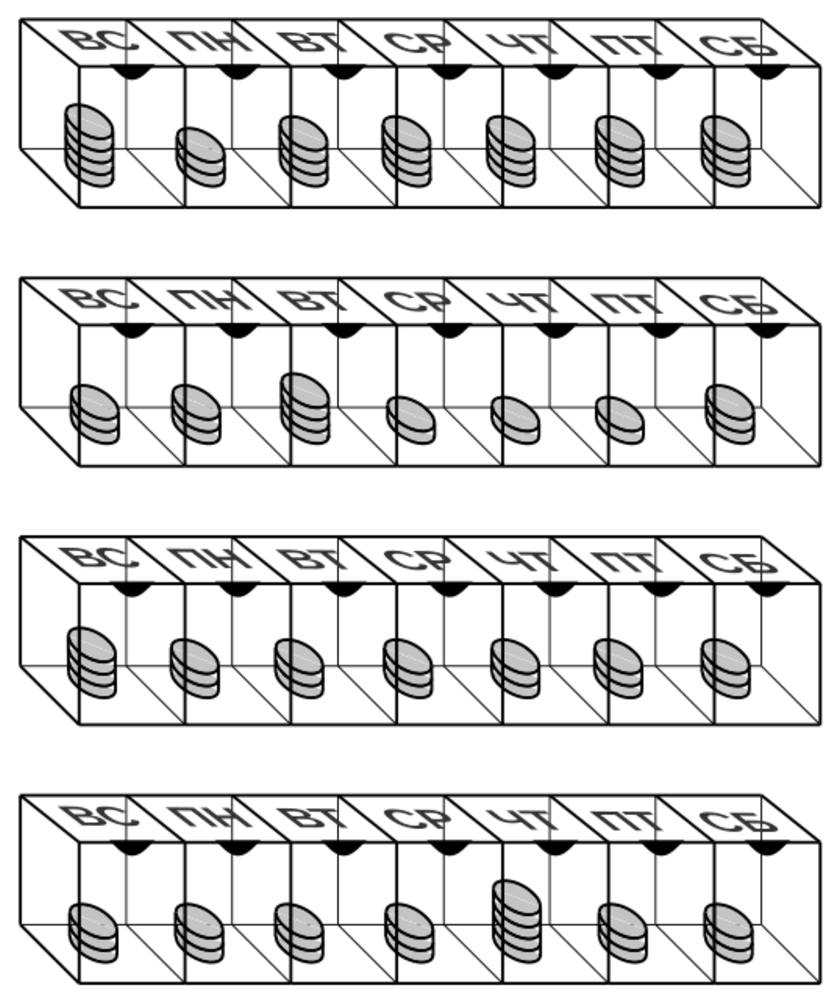
\includegraphics[scale=0.5]{Figs/Handicaps/box1-ru}
\end{figure}

Первая ячейка вправо от кучи, содержащая $k-1$ таблеток, будет той, из которой нужно взять таблетку.
Если ячейки с $k-1$ таблетками нет, тогда нужно взять таблетку из кучи.
В почти всех случаях надпись на ячейке, из которой берётся таблетка, правильная, то есть совпадает с текущим днём недели.

Например, коробочки на рисунке выше подготовлены для приёма таблетки во вторник, субботу, понедельник и четверг, соответственно.

Исключением является момент, когда у профессора остаётся последняя таблетка.
В предыдущий день он обнаружил две оставшиеся таблетки вместе в ячейке, помеченной соответствующим днём недели, и он одну оттуда взял (согласно правилу, что если нет ячейки размером на один меньше, чем куча, надо брать из кучи).
Теперь последняя таблетка лежит в ячейке, помеченной \emph{вчерашним} днём, и эту таблетку он принимает сегодня.

Легко заметить, что если таблетки разложены должным образом, тогда их конфигурация сохраняет верность правилам до последней таблетки.
Но всегда ли возможно всё правильно настроить, когда приходят новые таблетки?
И да, действительно, существует единственная правильная конфигурация для любого данного числа таблеток и любого данного дня недели, то есть ровно так профессору следует раскладывать новые таблетки.
Профессор вычисляет день, когда должна быть принята последняя таблетка (а именно, вчерашний день недели плюс число таблеток по модулю 7,
предполагается, что сегодняшнюю таблетку он ещё не выпил).
Конечно, дни недели пронумерованы последовательно  по модулю 7, но не имеет значения, который день номер~1.

Если, скажем, в среду утром пришло 32 таблетки, то профессор знает, что последнюю таблетку надо будет принять в субботу (из ячейки \textsc{пт}!) Из этого следует, что ячейка \textsc{пт} содержит кучу.
Профессор кладёт шесть таблеток в \textsc{пт}, по четыре таблетки в \textsc{сб}, \textsc{вс}, \textsc{пн}, \textsc{вт}, и по пять в \textsc{ср} и \textsc{чт}.
И теперь у него всё устроено должным образом, чтобы принять таблетку за среду.
\heart

Уместно спросить:
«А что, если у нас меньше, чем семь ячеек?
При каком наименьшем числе ячеек наша задача имеет решение?
А что, если в неделе $d$ дней, вместо семи,
каково тогда наименьшее возможное число ячеек, как функция от $d$?»

Отметим, что профессорское решение работает и на Юпитере, где в неделе $d$ дней ($d>1$), и где коробочки для таблеток, конечно же, имеют $d$ ячеек.
В случае $d=2$ это сводится к тому, что в одной ячейке держится на одну или две таблетки больше.
Решение для двух ячеек может быть использовано для любого чётного $d$, так как человек, принимающий таблетки, знает, какой сейчас день этой чётной недели, а значит он знает и чётность этого дня.
Так что наличие двух ячеек достаточно и, конечно, необходимо, если $d$ чётно.

Однако, две ячейки не сработают, если $d$ нечётно.
В этом случае непременно найдутся два последовательных дня недели, которые должны сойтись к одной однотаблеточной конфигурации, так что, когда человек видит такую конфигурацию в первый из этих дней, он не может сказать, принял ли он таблетку в этот день или нет.

Читателю, прошедшему уже такой долгий путь, не составит труда убедить себя, что при нечётных $d$ достаточно трёх ячеек.
Но придумать простой алгоритм с тремя ячейками для семидневной недели довольно сложно.
Предложенная далее схема основана не мнемоническом использовании двоичной записи.

Пронумеруем дни недели, начиная с воскресенья = 1 и заканчивая субботой = 7, числами по модулю 7.
Схема включает в себя семь «типов конфигураций», пронумерованных от 1 до 7, а конфигурации в каждом типе определяются по бинарному представлению номера типа.
При этом мы считаем, что ячейки располагаются в линейном порядке --- «левая», «центральная» и «правая» (то есть циклический порядок использоваться не будет).

Так, например, тип $1=001_2$ требует, чтобы правая ячейка была задействована как куча с гораздо б\'{о}льшим количеством таблеток, чем будет в каждой из двух остальных.
Тип $3 = 011_2$ требует, чтобы в левой ячейке было существенно меньше таблеток, чем в любой из двух остальных ячеек,
а тип 7$ = 111_2$ --- чтобы ячейки были более-менее равными.

Точнее, типы 1, 2 и 4 имеют кучи (справа, в центре и слева, соответственно), в которых на две или три таблетки больше, чем в любой из двух других ячеек.
При этом оставшиеся две ячейки, если они различны, то упорядочены так, что б\'{о}льшая ячейка находится правее.

Далее, типы 3, 5 и 6 имеют особую наименьшую ячейку слева, в центре или справа, соответственно.
Две другие ячейки содержат каждая на две таблетки больше, если они одинаковые.
Если нет, то они различаются по размеру не больше, чем на одну таблетку, и б\'{о}льшая ячейка расположена правее и содержит на 2 или 3 таблетки больше, чем самая маленькая.

Тип 7 требует, чтобы содержимое ячеек отличалось друг от друга максимум на одну таблетку, с меньшими ячейками справа (см. таблицу).

Теперь стратегия: если в день $D$ получено $P$ таблеток, то они распределяются согласно типу $P+D \pmod 7$.
Таблетки берутся так, чтобы сохранялся тип.

В частности, каждый день, профессор, смотрит на тип $T$ и поступает следующим образом:
если в день $D$ он видит $P>3$ таблеток и $D+P\ne T\pmod 7$, значит, он уже в этот день таблетку принял.
В противном случае, он берёт таблетку из одной ячейки, так, чтобы сохранить тип конфигурации.

\begin{center}
  \begin{tabular}{ l | c c c c }
     & 3 таб. & 4 таб & 5 таб & 6 таб \\ \hline
    тип 1 & 003 & 013 & 113 & 114 \\ 
    тип 2 & 030 & 031 & 131 & 141 \\ 
    тип 3 & 012 & 022 & 023 & 123\\ 
    тип 4 & 300 & 301 & 311 & 411\\ 
    тип 5 & 102 & 202 & 203 & 213\\ 
    тип 6 & 120 & 220 & 230 & 231\\ 
    тип 7 & 111 & 211 & 221 & 222
  \end{tabular}
\end{center}

Когда же останется три таблетки или меньше, становится трудно следовать какому-либо типу, но можно воспользоваться правилом «слева-направо» для типов, чтобы решать, как необходимо менять дальше конфигурации.
Это сводится к использованию следующей таблицы:

\begin{figure}[h!]
\centering
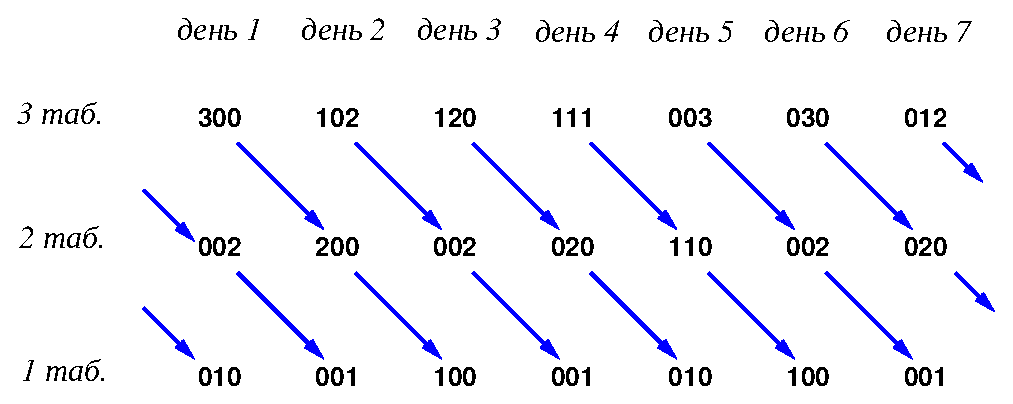
\includegraphics[scale=0.6]{Figs/Handicaps/3box-ru}
\end{figure}

Чтобы воспользоваться таблицей, нужно найти в ней запись, соответствующую $D$ и $P$;
если такая имеется, то нужно взять таблетку так, чтобы после получилась конфигурация ниже и направо (следуя по диагонали).
В противном случае, конфигурация будет соответствовать дню $D+1$, и, значит, таблетка за этот день уже принята.
